
            \documentclass{article}
            \usepackage{enumitem}
            \usepackage{roboto}
            \linespread{1.5}
            \usepackage{xcolor}
            \usepackage{longtable}
            \usepackage{pgf-pie}
            \usepackage[table]{xcolor}
            \usepackage{colortbl}
            \usepackage{graphicx}
            \usepackage{geometry}
            \usepackage{hyperref}
            \usepackage{fancyhdr}
            \usepackage{lastpage}
            \usepackage{tcolorbox}
            \usepackage{tikz}
            \usepackage{background}
            \usetikzlibrary{calc}
            \usetikzlibrary{fadings}
            \usepackage{titletoc}
            \usepackage{adjustbox}
            \usepackage{subfigure}
            \usepackage{pagecolor}
            \usepackage{titletoc}
            \usepackage[T1]{fontenc}
            \usepackage[scaled]{uarial}
            \usetikzlibrary{pie, fit}
            \usepackage[calc,useregional]{datetime2}
            \usepackage{datetime}
            \usepackage{array}
            \usepackage{wheelchart}
            \usetikzlibrary{decorations.markings}
            \usepackage{siunitx}
            \usepackage{eso-pic}
            \usetikzlibrary{shapes.geometric, positioning}
            \definecolor{darkgray}{RGB}{64,64,64}
            \definecolor{tablecol}{RGB}{54,127,140}
            \definecolor{tableco2}{RGB}{140,207,183}
            \definecolor{textbold}{RGB}{9,62,82}
            \definecolor{lightgray}{RGB}{245, 245, 245}
            \definecolor{textcolor}{RGB}{9,62,82}
            \definecolor{sectioncolor}{RGB}{5, 38, 37}
            \definecolor{subsectioncolor}{RGB}{64,110,140}
            \definecolor{critical}{RGB}{192,0,0}
            \definecolor{high}{RGB}{255,0,0}
            \definecolor{medium}{RGB}{255,192,0}
            \definecolor{low}{RGB}{146,208,80}
            \definecolor{info}{RGB}{242,242,242}
            \definecolor{total}{RGB}{218,238,243}
            \definecolor{shadow}{RGB}{227,227,227}
            \definecolor{infotext}{RGB}{0,176,240}
            \definecolor{linkColor}{RGB}{110,178,184}
            \usepackage{helvet}
            \renewcommand{\rmdefault}{phv}
            \renewcommand{\sfdefault}{phv}
            \usepackage{xurl}
            \usepackage{hyphenat}
            \urlstyle{same}


            \hypersetup{
                hidelinks,  
                colorlinks=false,
            }


            \newcommand{\urlstring}[1]{\begin{quote}\url{#1}\end{quote}}
            

            
            \color{textcolor}
            
            \pagecolor{white}
            \pagestyle{fancy}
            \fancyhf{}
            \fancyheadoffset[R]{0cm}
            \fancyhead[R]{\includegraphics[width=.18\textwidth]{vapt.jpeg}}
            \fancyfoot[R]{\textbf{\thepage}}
            \fancyfoot[c]{ \textbf{Company Confidential}} 
            \fancyfoot[l]{ \textbf{VAPTlabs Report}} 
            \renewcommand{\headrulewidth}{0pt}
            \renewcommand{\footrule}{\hspace{-2cm}\makebox[\dimexpr\paperwidth\relax]{\rule{\dimexpr\paperwidth-1.5cm}{1.0pt}} }
           

            
            \fancypagestyle{plain}{
            \fancyhf{} 
            \fancyhead{} 
            \renewcommand{\headrulewidth}{0pt}
            \fancyfoot[R]{\textbf{\thepage}}
            \fancyfoot[c]{ \textbf{Company Confidential}} 
            \fancyfoot[l]{ \textbf{VAPTlabs Report}}   
            }

            \thispagestyle{plain}
            \newcommand{\piechartRadius}{3}
      
            \geometry{
                left=2.0cm,
                right=2.0cm,
                top=3cm,
                bottom=3cm,
            }

            

            \backgroundsetup{
                scale=1,
                angle=0,
                opacity=1,
                color=black,
                contents={
                    
\begin{tikzpicture}[remember picture, overlay] 
                    \draw[line width=1pt] ($(current page.north west)+(0.3in, -0.3in)$) rectangle ($(current page.south east)+(-0.3in, 0.3in)$);
                    \end{tikzpicture}
                    }
                }

            \newcommand{\PageBorder}{
                
\begin{tikzpicture}[remember picture, overlay]
                    \draw[line width=1pt] ($(current page.north west)+(0.3in, -0.3in)$) rectangle ($(current page.south east)+(-0.3in, 0.3in)$);
                \end{tikzpicture}
            }

            \AddToShipoutPictureBG{\PageBorder}

            \makeatletter
            \renewcommand{\section}{\@startsection{section}{1}{\z@}%
            {-1ex \@plus -.1ex \@minus -.01ex}%
            {1.0ex \@plus  .01ex}%
            {\normalfont\large\bfseries\color{sectioncolor}}}

            
            \renewcommand{\subsection}{\@startsection{subsection}{2}{\z@}%
            {-.5ex\@plus -.1ex \@minus -.01ex}%
            {1.0ex \@plus .01ex}%
            {\normalfont\large\color{subsectioncolor}}}
            \makeatother


            \renewcommand{\contentsname}{Table of Contents}
            \titlecontents{section}
            [15pt] 
            {} 
            {\contentslabel{2em}}
            {} % numberless format
            {\titlerule*[0.5pc]{.}\contentspage}

            \renewcommand{\@}{\space\ignorespaces}

            \begin{document}


            \begin{minipage}{.30\textwidth}
            \begin{center}
            \includegraphics[width=.8\textwidth]{vapt.jpeg} 
            \end{center}
            \end{minipage}
            \begin{minipage}{.60\textwidth}
            \begin{flushleft}
                \huge Google Web Application Security Assessment Report.
            \end{flushleft}                
            \end{minipage}
            \vspace{80pt}

            \large Google Web Application
            \begin{tcolorbox}[colback=blue!10!white,colframe=white,width=1.0\textwidth,height=5pt]
            \end{tcolorbox}
            

            \begin{minipage}{.40\textwidth}
            \textbf{REPORT PUBLISH DATE}
            \end{minipage}
            \begin{minipage}{.60\textwidth}
            \textbf{
            \dayofweekname{\day}{\month}{\year}
            \shortmonthname[\month] 
            \the\day \
            \the\year \
            \currenttime~GMT+0000~(UTC)
            }
            \end{minipage}


            \vfill
            \clearpage
            \title{\large Bug Report Summary}
            
            \tableofcontents
            \newpage
            \section{\large Executive Summary}
                \subsection{\large Strategic Recommendation }
                \large It is recommended to fix all critical, high and medium vulnerabilities before releasing the application to
                    customer.
                \subsection{\large Scope of Work}
                \normalsize The scope of this penetration test was limited to the URL mentioned below: 
                    \begin{center}
                        \begin{longtable}[l] {|p{4em}|p{10em}|p{10em}|p{18em}|}
                        \hline 
                        \multicolumn{4}{|p{45.7em}|}{\large \cellcolor{tablecol} \textcolor{white}{\textbf{Scope Details}}} \\
                        \hline
                        \normalsize \cellcolor{tableco2} \textbf{Sr. No.} & \normalsize \cellcolor{tableco2} \textbf{Application Name} & \normalsize \cellcolor{tableco2} \textbf{Application URL} & \normalsize \cellcolor{tableco2} \textbf{Scope}  \\    
                        \hline
                        \normalsize 1. & \normalsize Google & \normalsize \url{www.google.com} & \normalsize Google Web Application Manually \& using Burpsuite \\
                        \hline
                        \end{longtable} 
                    \end{center}  
                    
                \subsection{\large Summary of Findings}
                \begin{itemize}[noitemsep]
                    \item \large Graphical Summary
                \end{itemize}
                
                \begin{minipage}{.55\textwidth}
                \normalsize \textbf{Vulnerability v/s Severity Pie Chart} 
                \end{minipage}
                \begin{minipage}{.40\textwidth}
                \normalsize \textbf{Vulnerability Summary}                
                \end{minipage}

                \vspace{20pt}
                \begin{minipage} {0.50\textwidth}                     
                \begin{tcolorbox}[colback=blue!10!white,colframe=white,width=0.85\textwidth]
                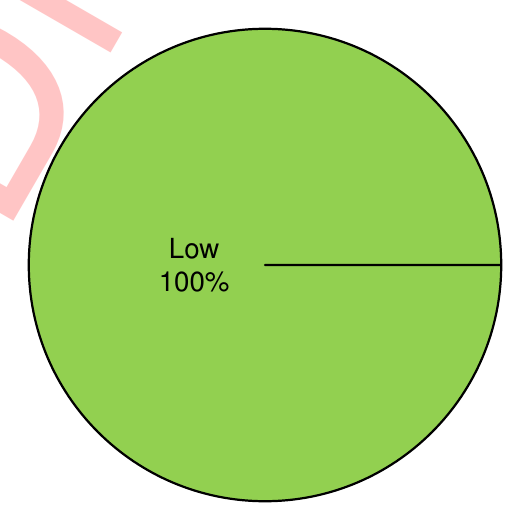
\begin{tikzpicture}
                \centering
                \pie[color={low}, text=inside, radius=\piechartRadius]{
                    100/Low
                }
                \end{tikzpicture}

                \begin{minipage} {.025\textwidth}
                \colorbox{critical}{}
                \end{minipage}
                \begin{minipage} {.17\textwidth}
                Critical
                \end{minipage}
                \begin{minipage} {.025\textwidth}
                \colorbox{high}{}
                \end{minipage}
                \begin{minipage} {.12\textwidth}
                High
                \end{minipage}
                \begin{minipage} {.025\textwidth}
                \colorbox{medium}{}
                \end{minipage}
                \begin{minipage} {.20\textwidth}
                Medium
                \end{minipage}
                \begin{minipage} {.03\textwidth}
                \colorbox{low}{}
                \end{minipage}
                \begin{minipage} {.11\textwidth}
                Low
                \end{minipage}
                \begin{minipage} {.02\textwidth}
                \colorbox{info}{}
                \end{minipage}
                \begin{minipage} {.14\textwidth}
                Info
                \end{minipage}
                
                \end{tcolorbox}
                \end{minipage}
                \begin{minipage}{.40\textwidth}
                \renewcommand{\arraystretch}{1.63}
                \begin{tabular}{|p{11em}|>{\centering\arraybackslash}p{6em}|}
                \hline
                \normalsize \cellcolor{black!10} \textbf{Severity} & \normalsize \cellcolor{black!10} \rule{0pt}{5ex} \textbf{Count} \\
                 \hline
                 \normalsize Critical &   \normalsize \cellcolor{critical} 0  \\
                 \hline
                 \normalsize High & \normalsize \cellcolor{high}  0 \\
                 \hline
                 \normalsize Medium & \normalsize \cellcolor{medium}  0 \\
                 \hline
                 \normalsize Low & \normalsize \cellcolor{low}  1 \\
                 \hline
                 \normalsize Informational & \normalsize \cellcolor{info} 0 \\
                 \hline
                 \normalsize Total & \normalsize \cellcolor{total} \rule{0pt}{4ex} 1 \\
                 \hline    
                \end{tabular}
                \end{minipage}

 

            \newpage
            \section{\large CVSS: Score Vulnerabilities}
            \large there are three types of scores that can be calculated: a base score, a temporal score and an environmental score. For purposes of reporting in this document, the CVSS base score will be provided. The base score assesses the following characteristics:
            \begin{center}
                \begin{longtable} {|p{9em}|p{31em}|}
                \hline 
                \large \cellcolor{tablecol} \textcolor{white}{\textbf{Characteristics}} & \large \cellcolor{tablecol} \textcolor{white}{\textbf{Description}}   \\    
                \hline
                \normalsize Attack Vector & \normalsize Assesses whether or an adversary can mount attack from a remote network, a local
                network or if an adversary must be logged on to the target of evaluation or physically
                connected.  \\
                \hline
                \normalsize Attack Complexity  & \normalsize Assesses the complexity of an attack dependent on how many of the attack variables are
                within the control of the adversary.  \\
                \hline
                \normalsize Privileges Required  & \normalsize Assesses the level of access that an attacker needs to mount a successful attack. \\
                \hline
                \normalsize User Interaction & \normalsize Assesses the extent to which actions of the victim are required for an attack to be
                successful. \\
                \hline
                \normalsize Scope & \normalsize Assess whether the impact of an attack is limited to the target of evaluation or if the attack
                has impact on other systems as well. \\
                \hline
                \normalsize Confidentiality & \normalsize Assesses the negative impact that an attack can have on the target of evaluation's
                confidentiality. \\
                \hline
                \normalsize Integrity & \normalsize Assesses the negative impact that an attack can have on the target of evaluation's
                integrity. \\
                \hline
                \normalsize Availability & \normalsize Assesses the negative impact that an attack can have on the target of evaluation's
                availability. \\
                \hline
                \end{longtable}   
            \end{center} 

            \noindent \large As indicated above, the assessment of these characteristics results in a severity score which ranges
            from 1-10. This score can be further broken down into the following rating levels: \\
            \newpage
            \begin{center}
                \begin{longtable} {|p{4.5em}|p{4.5em}|p{30em}|}
                \hline 
                \large \cellcolor{tablecol} \textcolor{white}{\textbf{Range}} & \large \cellcolor{tablecol} \textcolor{white}{\textbf{Rating}} & \large \textcolor{white}{\cellcolor{tablecol} \textbf{Description}}   \\    
                \hline
                \normalsize \textbf{9.0 - 10.0} & \normalsize \textcolor{critical}{\textbf{Critical}} & \normalsize These types of vulnerabilities should be reviewed immediately for impact to the
                business. This rating usually indicates that an exploit exists that could easily be use
                severely impact confidentiality, integrity and/or availability.  \\
                \hline
                \normalsize \textbf{7.0 - 8.9} & \normalsize \textcolor{high}{\textbf{High}} & \normalsize These types of vulnerabilities need to be assessed in the short term for impact to the
                business. A score in this range indicates that a vulnerability could be exploited with
                low to medium complexity and could have moderate or high impact on confidentiality,
                integrity and/or availability.  \\
                \hline
                \normalsize \textbf{4.0 - 6.9} & \normalsize \textcolor{medium}{\textbf{Medium}} & \normalsize These vulnerabilities should also be evaluated for impact to the business, but the
                base score shows that these types of vulnerabilities may be only exploitable with
                increased effort or have little impact to confidentiality, integrity and/or availability.  \\
                \hline
                \normalsize \textbf{0.1 - 3.9}  & \normalsize \textcolor{low}{\textbf{Low}} & \normalsize These vulnerabilities should also be evaluated, but from evaluating the base
                characteristics, the exploitation of these vulnerabilities is likely to result in little
                negative impact to confidentiality, integrity and/or availability.  \\
                \hline
                \end{longtable}   
            \end{center}
            \large The CVSS score provided in this report is meant to serve as a tool to assist with the prioritizing
            vulnerability resolution. This score, however, does not take into consideration the context of the
            business. For some business IT contexts some lower-scored vulnerabilities could have serious
            business impact. Hence, all of the reported vulnerabilities should be taken into consideration.

            \subsection{\large How to use this report}

            \large The vulnerabilities reported in this document provide a view of the target of evaluation's security posture
            at the time of testing. This timeframe, "at the time of testing", is important to highlight because the report
            cannot address future changes to the target of evaluation, changes in the systems that support the target of evaluation and emerging, publicly disclosed exploits that could have an impact on the target
            of evaluation.

            \noindent \large The goal of this document is to provide input to help identify and prioritize the vulnerabilities that were
            detected at the time of testing and to provide some guidance as to how the vulnerabilities might be
            mitigated.
            
            \begin{center}
                \begin{longtable} {|p{9em}|p{31em}|}
                \hline 
                \large \cellcolor{tablecol} \textcolor{white}{\textbf{Characteristics}} & \large \cellcolor{tablecol} \textcolor{white}{\textbf{Description}}   \\    
                \hline
                \normalsize Status & \normalsize This field will contain either "Verified" or "Detected". If this value is "Verified", then the tester exploited this vulnerability during the penetration test. If it is "Detected",
                then evidence of the vulnerability was found, but it was not exploited during testing. There are many reasons why a tester may not be able to exploit a vulnerability
                during testing. Examples include threat of system instability after exploit, lack of time during testing and/or inability to find a vector by which a vulnerability could be exploited.  \\
                \hline
                \normalsize CVSSv3.1 Scoring  & \normalsize This provides the overall severity score for a vulnerability including the individual
                assessments for attack vector, attack complexity, privileges required, user interaction, scope, confidentiality, integrity and availability.  \\
                \hline
                \normalsize Vulnerability Description  & \normalsize This provides an overview of the identified vulnerability including how it could be useful to an adversary. \\
                \hline
                \normalsize Proof of Concept & \normalsize This provides a description of how the vulnerability was detected and/or a description of how it can be reproduced for testing purposes. \\
                \hline
                \normalsize Affected Uri  & \normalsize This provides a list of the url that are relevant to the vulnerability. \\
                \hline
                \normalsize Recommendation & \normalsize This provides suggestions on how to mitigate the vulnerability. \\
                \hline
                \normalsize References & \normalsize This provides links to CVEs, CWEs and other known resources to learn more about the vulnerability and how to mitigate the vulnerability. \\
                \hline
                \end{longtable}   
            \end{center}
            
            \noindent \large The report is broken up into three major sections: an executive summary, a technical detail report and an appendix. The executive summary will provide a high-level overview of the vulnerabilities detected
            during the penetration test.

            \noindent \large The technical detail report will provide the details of the vulnerabilities identified during the penetration test. Each vulnerability will include the following descriptors.
            
            \noindent \large The appendix will contain information about the testing environment and further details gathered during testing that do not fit within the first three chapters. 
            This information is necessary to have a complete picture of the penetration test, but it is in the appendix to make accessing the testing results more userfriendly.


            \newpage
            \section{\large Findings Overview}
            \ \  \ The following table summarizes the list of findings discovered during the security assessment
            \begin{center}
                \begin{longtable} {|p{2em}|p{20em}|>{\raggedright\arraybackslash}p{7em}|>{\centering\arraybackslash}p{4em}|>{\centering\arraybackslash}p{3em}|}
                    \hline 
                    \multicolumn{5}{|p{40.2em}|}{\large \cellcolor{tablecol} \textcolor{white}{\textbf{Summary Table}}} \\
                    \hline
                    \normalsize \cellcolor{tableco2} \textbf{Sr. No.} & \normalsize \cellcolor{tableco2} \textbf{Vulnerability Name} & \normalsize \cellcolor{tableco2} \textbf{OWASP Category} & \normalsize \cellcolor{tableco2} \textbf{Severity} & \normalsize \cellcolor{tableco2} \textbf{CVSS Score++} \\    
                    \hline
                    
                    \normalsize \center 1 & \normalsize as & \normalsize A05-Security Misconfiguration  & \normalsize \textbf{\textcolor{infotext}{Info}} &  3 \\
                    \hline
                     
                \end{longtable}   
            \end{center}
            
            
            \newpage
            \section{\large Technical Reports}
            \ \ \ The following findings were made during the assessment.    
            \begin{center}
                \begin{longtable}{|p{30em}|p{10em}|}
            \hline
            \textbf{Finding Name} & \textbf{Remediation Effort}  \\
            \hline
            \multicolumn{2}{|p{20em}|}{\normalsize \textcolor{critical}{\textbf{Critical Severity Findings}}} \\
            \hline
            
        \multicolumn{2}{|p{20em}|}{\normalsize \textcolor{high}{\textbf{High Severity Findings}}} \\
        \hline
    
        \multicolumn{2}{|p{20em}|}{\normalsize \textcolor{medium}{\textbf{Medium Severity Findings}}} \\
        \hline
    
        \multicolumn{2}{|p{20em}|}{\normalsize \textcolor{low}{\textbf{Low Severity Findings}}} \\
        \hline
    
        \multicolumn{2}{|p{20em}|}{\normalsize \textcolor{infotext}{\textbf{Informational Findings}}} \\
        \hline
    
     as &  Planned \\
    \hline\end{longtable}
            \end{center}
            
                    \newpage
                    \subsection{\large as}
                    \begin{description}[itemsep=2pt, leftmargin=0.2cm]
                        \item \large \textbf{Status:} New
                        \item \large \textbf{Severity: \textcolor{infotext} {Info}}
                        \item \large \textbf{OWASP Category: A05-Security Misconfiguration}
                        \item \large \textbf{CVSS Score:} 3 
                        \item \large \textbf{Affected Hosts/URLs:}
                            \begin{itemize} 
                            \item \large \url{as}
                            \end{itemize}
                        \item \large \textbf{Summary:} \\  \large sa
                            
                        \item \large \textbf{Screenshot:} \\ \\
                        \includegraphics[width=1.0\textwidth,height=0.5\textheight,keepaspectratio]{Images/temp-image-0-0.png} \\
                       

                        \item \large \textbf{Steps of Reproduce:}
                        \linespread{1.0}
                        \begin{enumerate}[leftmargin=0.5cm]
                            
                        \item \large sde
                        \end{enumerate}
                        
                        \item \large \textbf{Impact:}
                        \linespread{1.0}
                        \begin{enumerate}[leftmargin=0.5cm]
                        \item \large sd 
                        \end{enumerate}  
                
                
                        \item \large \textbf{Remediation:}
                        \linespread{1.0}
                        \begin{enumerate}[leftmargin=0.5cm]
                            
                        \item \large ds
                        \end{enumerate}

                        \item \large \textbf{Reference:}
                        \linespread{1.0}
                        \begin{enumerate}[leftmargin=0.5cm ]
                            
                        \item \large \textcolor{linkColor}{\url{ds}}
                       
                        \end{enumerate}   
                    \end{description}
                    
                    
            \newpage
            \section{\large Annexures}
                \subsection{\large OWASP TOP 10:2021}

                \begin{center}
                \begin{longtable} {|>{\raggedright\arraybackslash}p{10em}|p{30em}|}
                \hline
                \multicolumn{2}{|p{41em}|} {\cellcolor{tablecol}\textbf{OWASP TOP 10:2021}} \\
                \hline
                \large \cellcolor{tableco2} \textbf{Name} & \large \cellcolor{tableco2} \textbf{Description} \\
                \hline
                \normalsize \textbf{A01:2021-Broken Access Control} & 
                \normalsize Access control enforces policy such that users cannot act outside of their intended
                permissions. Failures typically lead to unauthorized information disclosure, modification,
                or destruction of all data or performing a business function outside the user's limits. \\
                \hline
                \normalsize \textbf{A02:2021-Cryptographic Failures} & 
                \normalsize Previously known as Sensitive Data Exposure, Cryptographic Failures involve protecting
                data in transit and at rest. This includes passwords, credit card numbers, health records,
                personal information, and business secrets that require extra protection, especially if that
                data falls under privacy. \\
                \hline
                \normalsize \textbf{A03:2021-Injection} & 
                \normalsize Injection flaws, such as SQL, OS, XXE, XSS and LDAP injection occur when untrusted
                data is sent to an interpreter as part of a command or query. The attacker's hostile data
                can trick the interpreter into executing unintended commands or accessing data without
                proper authorization. \\
                \hline
                \normalsize \textbf{A04:2021-Insecure Design(Currently out of scope) } & 
                \normalsize Insecure design is a broad category representing different weaknesses, expressed as
                "missing or ineffective control design." Secure design is a culture and methodology that
                constantly evaluates threats and ensures that code is robustly designed and tested to
                prevent known attack methods. \\
                \hline
                \normalsize \textbf{A05:2021-Security Misconfiguration} & 
                \normalsize Security misconfiguration is the most commonly seen issue. This is commonly a result of
                insecure default configurations, incomplete or ad hoc configurations, open cloud storage,
                misconfigured HTTP headers, and verbose error messages containing sensitive
                information. Not only must all operating systems, frameworks, libraries, and applications
                be securely configured, but they must be patched/upgraded in a timely fashion. \\
                \hline
                \normalsize \textbf{A06:2021-Vulnerable and Outdated Components} & 
                \normalsize Components, such as libraries, frameworks, and other software modules, almost always
                run with full privileges. If a vulnerable component is exploited, such an attack can facilitate
                serious data loss or server takeover. Applications using components with known
                vulnerabilities may undermine application defences and enable a range of possible attacks
                and impacts. \\
                \hline
                \normalsize \textbf{A07:2021-Identification and Authentication Failures} & 
                \normalsize Application functions related to authentication and session management are often
                implemented incorrectly, allowing attackers to compromise passwords, keys, or session
                tokens, or to exploit other implementation flaws to assume other users' identities
                (temporarily or permanently). \\
                \hline
                \normalsize \textbf{A08:2021-Software and Data Integrity Failures (Currently out of scope)} & 
                \normalsize Software and data integrity failures relate to code and infrastructure that does not protect
                against integrity violations. This new category is making assumptions related to software
                updates, critical data, and CI/CD pipelines without verifying integrity. \\
                \hline
                \normalsize \textbf{A09:2021-Security Logging and Monitoring Failures} & 
                \normalsize Insufficient logging and monitoring, coupled with missing or ineffective integration with
                incident response, allows attackers to further attack systems, maintain persistence, pivot
                to more systems, and tamper, extract, or destroy data. Most breach studies show time to
                detect a breach is over 200 days, typically detected by external parties rather than internal
                processes or monitoring. \\
                \hline
                \normalsize \textbf{A10:2021-ServerSide Request Forgery(SSRF)} & 
                \normalsize SSRF flaws occur whenever a web application is fetching a remote resource without
                validating the user-supplied URL. It allows an attacker to coerce the application to send a
                crafted request to an unexpected destination, even when protected by a firewall, VPN, or
                another type of network access control list (ACL). \\
                \hline
                \end{longtable}
                \end{center}


                \subsection{\large Tools Used}

                \begin{center}
                \begin{longtable} {|p{10em}|>{\raggedright\arraybackslash}p{30em}|}
                \hline
                \multicolumn{2}{|p{41em}|} {\cellcolor{tablecol} \textbf{Tools:}} \\
                \hline
                \large \cellcolor{tableco2} \textbf{Name} & \large \cellcolor{tableco2} \textbf{Description} \\
                \hline
                \normalsize \textbf{Burp suite} & \normalsize \textbf{Burp Suite is an integrated platform for attacking web applications.} \large http://portswigger.net/suite \\
                \hline
                \normalsize \textbf{Nmap} & \normalsize \textbf{Nmap is a network mapper tool to scan for SSL related vulnerabilities} \large https://nmap.org \\
                \hline
                \end{longtable}
                \end{center}   
            \end{document}